\section{Theorie}
\label{sec:theorie}

Werden Atome mit geeigneter Energie beschossen, lässt sich mithilfe
der Energieübergänge der Elektronen die Struktur der Elektronenhüllen aufklären. \\

Auf die gleiche Weise funktioniert auch das Franck-Hertz-Experiment,
bei dem im einem abgeschlossenen Raum monoenergetische Elektronen mit
Quecksilberdampf interagieren.
Die dabei auftretenden (un-)elastischen Stöße zwischen den Elektronen und Hg-Atomen
lassen sich verwenden, um die die vom Quecksilberatom aufgenommene Energie zu ermitteln. \\

Für den unelastischen Stoß, bei dem das Hg-Atom aus seinem Ruhezustand in den
ersten angeregten Zustand übergeht, gilt mit der Ruhemasse $m_0$
des Elektrons sowie $v_\text{vor}$ und $v_\text{nach}$ als Geschwindigkeiten
des Elektrons vor und nach dem Stoß

\begin{equation*}
    E_1 - E_0 = \dfrac{m_0 \, v^2_\text{vor}}{2} -\dfrac{m_0 \, v^2_\text{nach}}{2}
\end{equation*}

Das Experiment selbst ist dabei nach \autoref{fig:abb1} aufgebaut.

\begin{figure}[H]
    \centering
    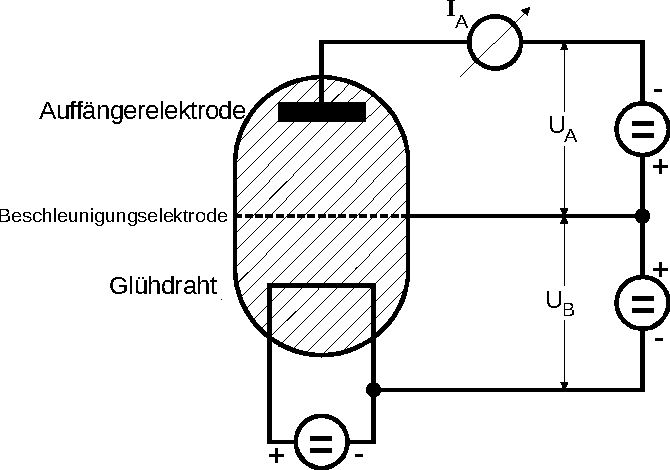
\includegraphics{figures/Abb_1.pdf}
    \caption{Schematischer Aufbau des Franck-Hertz-Versuches\cite{ap08}.}
    \label{fig:abb1}
\end{figure}

In Folge des glühelektrischen Effekts treten bei Erhitzung des Glühdrahts
ein Großzahl an Elektronen aus, die nach Durchlaufen der Beschleunigungsstrecke
eine kinetische Energie von

\begin{equation*}
    \dfrac{m_0}{2} v^2_\text{vor} = \text{e}_0 U_\text{B} \,,
\end{equation*}
wobei $\text{e}_0$ die Elementarladung der Elektronen und $U_\text{B}$
die an die Elektrode angelegte Gleichspannung darstellen. \\

Die Elektronen treffen auf die Auffängerelektrode, die der Beschleunigerelektrode gegenüber
die Gegenspannung $U_\text{A}$ besitzt. \\

Für die Geschwindigkeitskomponente $v_\text{z}$ in Feldrichtung gilt die Ungleichung
\begin{equation*}
    \dfrac{m_0}{2} v^2_\text{z} \geq \text{e}_0 U_\text{A} \,.
\end{equation*}
Alle Elektronen, die diese Ungleichung nicht erfüllen, kehren zur Beschleunigerelektrode zurück.
Dort können sie nun mit den Quecksilberatomen stoßen, wobei zwei Fälle unterschieden werden müssen. \\

Bei mittlerer Energie treten lediglich elastische Stöße auf, die
Energieabgabe $\Delta E$ beträgt dabei

\begin{equation*}
    \Delta E = \frac{4 m_0 M}{(m_0 + M)^2} E \approx 1,1 \cdot 10^{-5} E \,.
\end{equation*}

Ist die Elektronenenergie $E$ (durch Erhöhen der Beschleunigungsspannung $U_\text{B}$)
größer gleich der Energiedifferenz $E_1 - E_0$ zwischen erstem angeregten und Ruhezustand
des Hg-Atoms, überträgt es exakt diesen Energiebetrag an das Quecksilberatom. \\

Dieses fällt nach einer Relaxationszeit von $~10^{-8} \unit{\second}$
in seinen Ruhezustand zurück und emittiert ein Lichtquant der Energie
\begin{equation*}
    \text{h} \nu = E_1 - E_0
\end{equation*}

Wird nun der Auffängerstrom $I_\text{A}$ an der Auffängerelektrode
beobachtet, lässt sich feststellen, dass, wie in \autoref{fig:abb2} zu erkennen,
jähe Abnahmen des Stroms genau da finden, wo die Elektronen genug Energie besitzen,
um das Quecksilber anzuregen, aber nicht, um die Auffängerelektrode zu erreichen. \\

Dieser Vorgang lässt sich erneut beobachten, wenn die Elektronen erneut
eine Energie von $E_1 - E_0$ erreicht haben und ein weiteres Mal unelastisch mit
dem Hg stoßen können.

\begin{figure}[H]
    \centering
    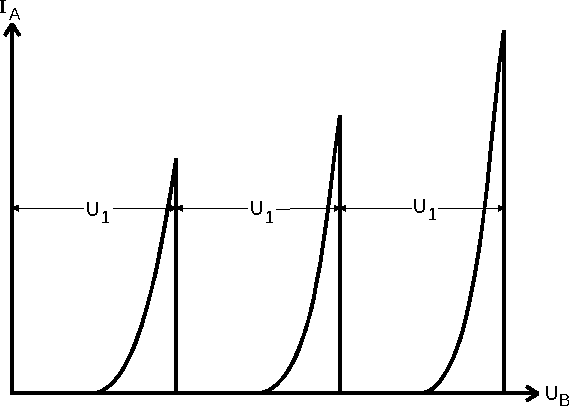
\includegraphics{figures/Abb_2.pdf}
    \caption{Zusammenhang zwischen Auffängerstrom $I_\text{A}$ und Beschleunigungsspannung $U_\text{B}$\cite{ap08}.}
    \label{fig:abb2}
\end{figure}

Der Abstand $U_1$ zwischen zwei Maxima beträgt dabei

\begin{equation}
    U_1 := \frac{1}{\text{e}_0} (E_1 - E_0) \,.
\end{equation} \\

Die in der Realität beobachtbare Kurve weicht jedoch von der in \autoref{fig:abb2} angegeben Kurve ab.
Dabei spielen insbesondere die drei folgenden Faktoren eine Rolle.

\subsection*{a) Das Kontaktpotential}

Um bereits bei niedrigen Temperaturen eine hohe Emissionsrate zu erzielen, wird für den Glühdraht ein Material
gewählt, dessen Austrittsarbeit $\Phi_\text{G}$ weit geringer als die Austrittsarbeit $\Phi_\text{B}$ der
Beschleunigerelektrode ist. \\

Wie in \autoref{fig:abb3} zu erkennen, entsteht so ein Potentialgefälle.

\begin{figure}
    \centering
    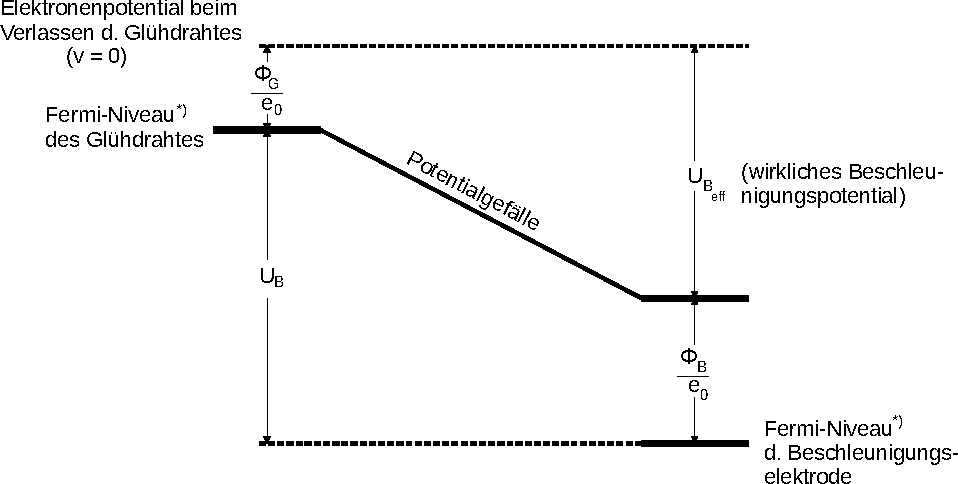
\includegraphics{figures/Abb_3.pdf}
    \caption{Potentialgefälle zwischen Glühdraht und Beschleunigungselektrode\cite{ap08}.}
    \label{fig:abb3}
\end{figure}

Das wahre Beschleunigerpotential
ist dann durch
\begin{equation*}
    U_{\text{B},\text{eff}} = U_\text{B} - \frac{1}{\text{e}_0} (\Phi_\text{B} - \Phi\text{G})
\end{equation*}
gegeben. \\

Der Ausdruck
\begin{equation*}
    K := \frac{1}{\text{e}_0} (\Phi_\text{B} - \Phi\text{G})
\end{equation*}
wird dabei als Kontaktpotential bezeichnet.


\subsection*{b) Das Energiespektrum der Elektronen}

Bei der Emission aus dem Glühdraht treten die Elektronen nicht, wie bisher angenommen, mit einheitlicher Energie aus.
Stattdessen besitzen sie bereits ein Energiespektrum (Fermi-Dirac-Verteilung), nach Durchlaufen des Beschleunigungspotential $U_\text{B}$
sind sie also energetisch verteilt. \\

Die unelastischen Stöße beginnen also nicht bei einer festgelegten Beschleunigungsspannung, sondern erstrecken
sich über einen endlichen Einsatzbereich. \\

Dadurch nähert sich die in \autoref{fig:abb2} dargestellte Kurve den Maxima weniger steil an und fällt nicht
unstetig, sondern stetig auf ein Stromminimum ab. \\

Die elastischen Stöße zwischen Elektronen und Quecksilberatomen spielen nur eine Rolle, wenn sie zwischen
Beschleunigungs- und Auffängerelektrode stattfinden.
Durch die Änderung in der z-Komponente der Elektronengeschwindigkeit kommt es zur Abflachung und Verbreiterung
der Franck-Hertz-Kurve.


\subsection*{c) Der Dampfdruck}

Für die Franck-Hertz-Kurve ist die Beobachtung der Zusammenstöße zwischen Elektronen und Quecksilberatomen
essentiell.
Damit diese in zufriedenstellender Anzahl auftreten, muss die mittlere freie Weglänge $\bar{w}$ der Elektronen
klein gegen den Abstand $a$ zwischen Kathode und Beschleunigungselektrode sein. \\

Über den Sättigungsdampfdruck $p_\text{sät}$ lässt sich die mittlere freie Weglänge durch
\begin{equation}
    \bar{w} [\unit{\centi\meter}] = \frac{0,0029}{p_\text{sät}} \left[\unit{\frac{1}{\milli\bar}} \right]
    \label{eq:mittfreiweg}
\end{equation}
bestimmen. \\

Der Sättigungsdampfdruck ist dabei temperaturabhängig, für Quecksilber ergibt sich mit
\begin{equation*}
    p_\text{sät} (T) = 5,5 \cdot 10^7 \text{e}^{-\dfrac{6876}{T}}
\end{equation*}
die in \autoref{fig:abb4} dargestellte Kurve.

\begin{figure}
    \centering
    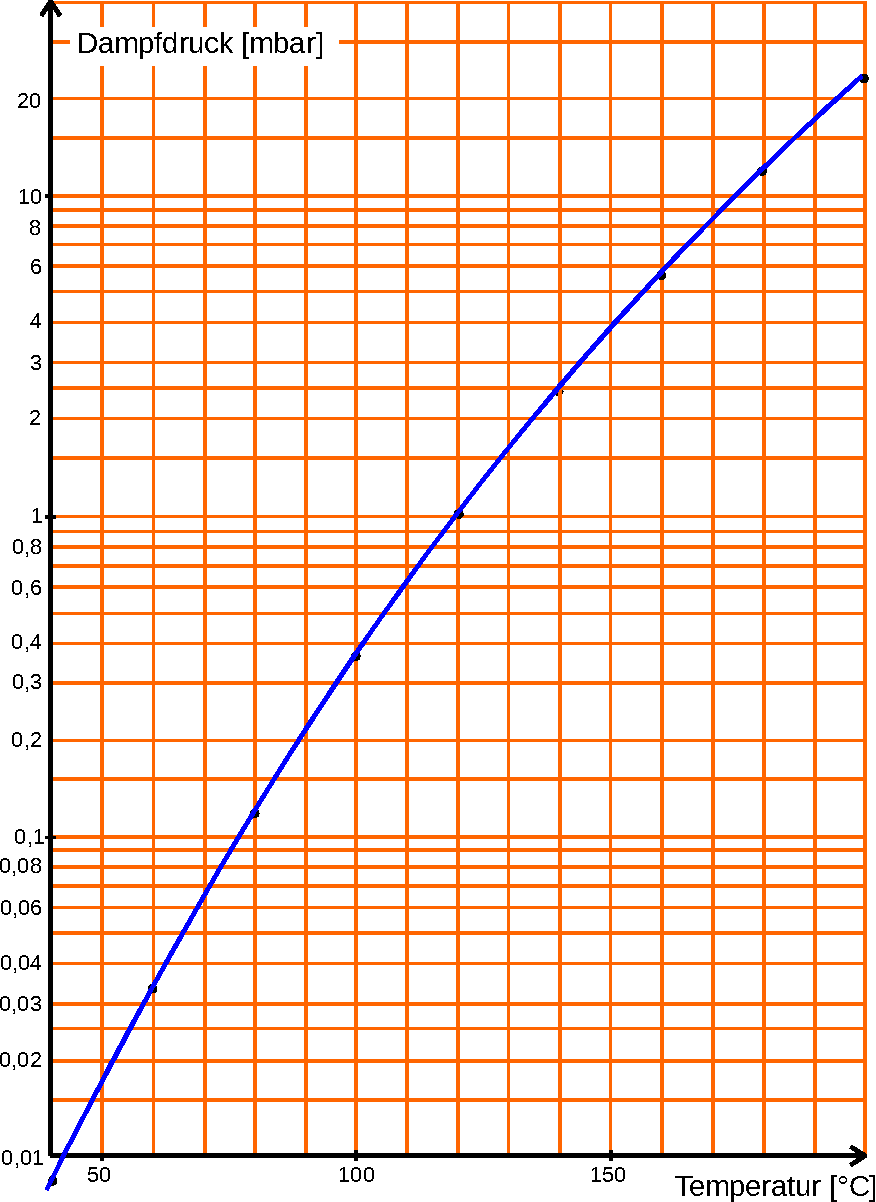
\includegraphics{figures/Abb_4.pdf}
    \caption{Dampfdruckkurve von Quecksilber\cite{ap08}.}
    \label{fig:abb4}
\end{figure}

So lässt sich eine Temperatur bestimmen, für die $\bar{w}$  $1000$ bis $4000$ Mal kleiner als $a$, die
Stoßwahrscheinlichkeit also ausreichend ist.

